\section{GPU Implementation} \label{sec:gpu} 

We implemented the new algorithm FastHASH in CUDA as well. Please note that
this is not a final implementation. Currently, we assign each graphic processor
one fragment. For each fragment, we then spawn 32 threads as a warp.  For each
thread, they have 2 phases in calculation. Phase 1 is the Adjacency Filtering
and phase 2 is edit-distance calculation. To keep as many threads in a warp as
possible, we synchronize all threads within one processor between 2 phases. The
flow chart is shown in Figure~\ref{fig:gpu}.  We have three main problems with
this naïve implementation. We will describe them below. \\

%%%%%%%%%%%%%%%%%%%%%%%%%%%%%%%%%%%%%%%%%%%%%%%%%%%%%%%%%%%%%%%%%%%%%%%%%%%%%%%%
\begin{figure}[t]
\centering
\vspace{0.1in}
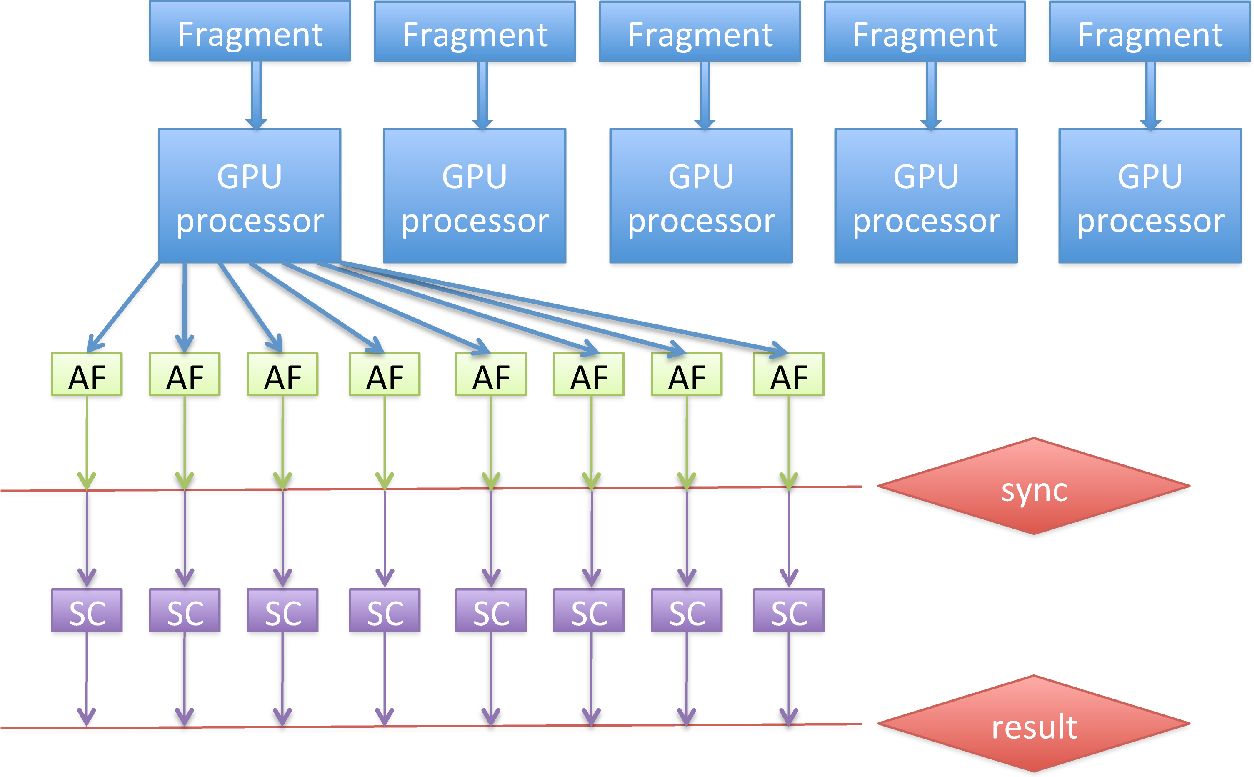
\includegraphics[width=3in]{./figure/gpu_B.pdf} \vspace{0in}
\caption{GPU flow chart}
\label{fig:gpu}
\end{figure}
%%%%%%%%%%%%%%%%%%%%%%%%%%%%%%%%%%%%%%%%%%%%%%%%%%%%%%%%%%%%%%%%%%%%%%%%%%%%%%%%

One problem we face in our CUDA implementation is that the edit distance
calculation diverges a lot in control path. This is because the algorithm we
implement is a lazy path filling algorithm* which tries to reduce work as much
as possible. Such reduction introduced a huge amount of divergence, since each
path may differ in ending point and they make the cheapest decisions based on
previous execution result. Divergence hurt GPU drastically since all the
threads within a warp have to always execute both paths. \\

Another problem with GPU is that for each fragment, the number of coordinates
that passes through Adjacency Filtering differs a lot. For a 32 threads warp,
to reach its maximum performance, we would like to have 32 threads working on
edit distance calculations at the same time. As a result, in order to
efficiently uses GPU, we would like each fragment has a multiple of 32
coordinates passes Adjacency Filtering, which, as we will show later in
evaluation section, is not true for real workload. In fact, the real workload
is a lot worse. For most of the time, the warp cannot be even filled up. One
way to fix this problem, as we are still exploiting, is to bind multiple
fragments to 1 processor, thus increasing the coordinates number that pass
Adjacency Filtering and subject to edit-distance calculation. \\

The third problem is that currently we are statically distributing workload. We
assign all processor the same amount of fragments to align. Again, due to the
intrinsic difference in edit-distance cost and adjacency filtering cost for
each fragment, the total work and execution time for each processor varies.
However, since we have to wait for the last processor to finish, the slowest
processor will dominate the execution time. We may solve this problem by
designing a smarter scheduler that dynamically redistributes fragments.\\
